\section{Lidar detection range analysis}
It is useful to know possible range of detection based on lidar sensor. This range influences the way how the waypoints for exploration are generated. Higher the detection range is, lower number of waypoints is necessary for exploring whole arena. There is a limited time for exploration, because brick pickup and brick placement takes a lot of time. Speed of pickup and placement is limited mainly by the speed of Kinova arm. We estimate the maximal range using the figure \ref{fig:range}.

\begin{figure}[H]
\centering
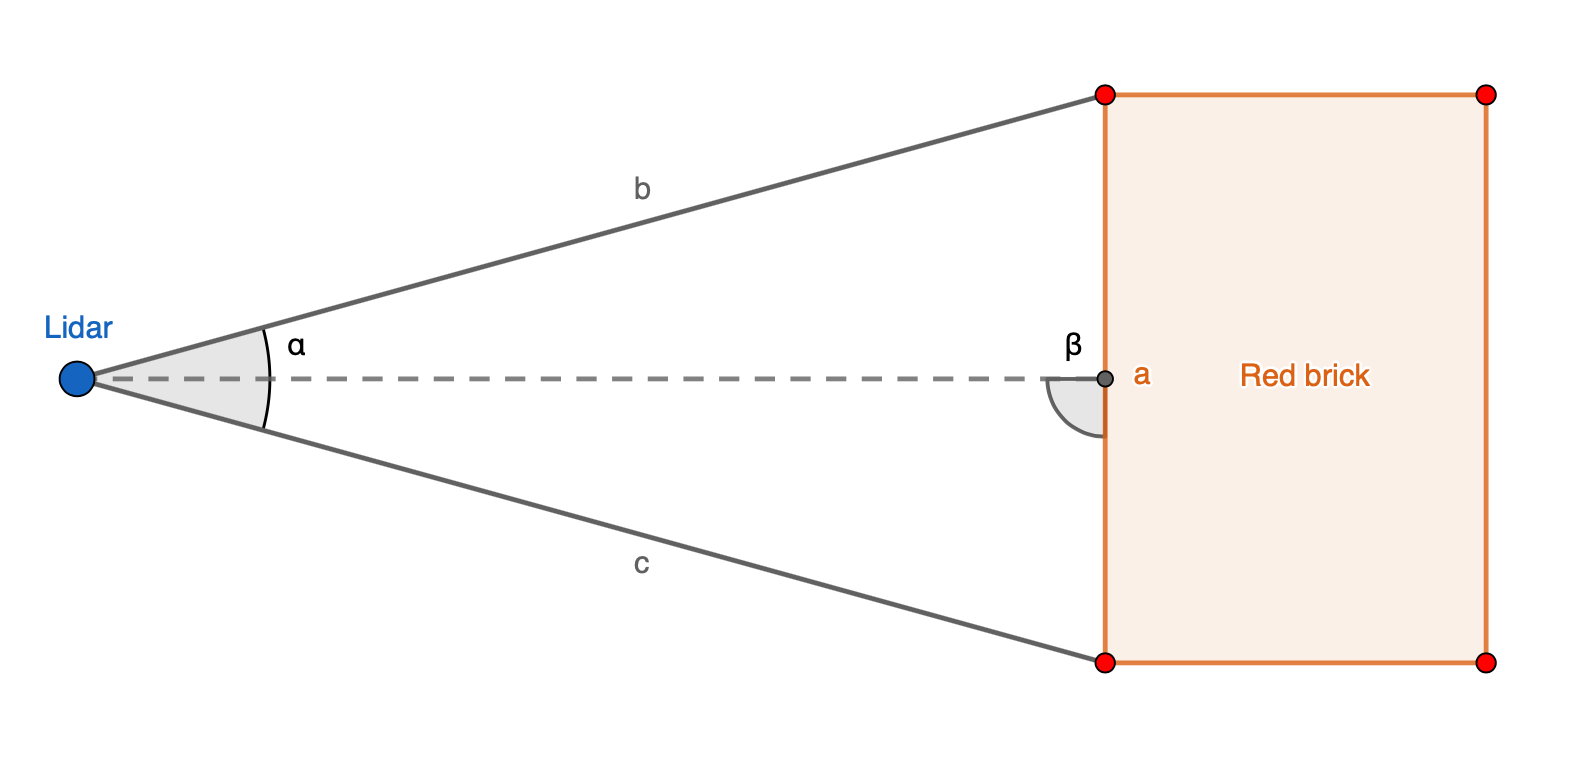
\includegraphics[scale=1.1]{fig/lidar_range.png}
\caption[Lidar range study]{Visualization of rays hitting the red brick.}
\label{fig:range}
\end{figure}

Angle $\alpha$ is the resolution of lidar known from table \ref{tab:lidar}. Only the maximal range is calculated thus angle $\beta = 90\degree$. To obtain the distance between points on the brick the cosine theorem can be used.
\begin{equation}
a^2 = b^2 + c^2 - 2bc \cos \alpha.
\end{equation}
Because $\beta$ is right angle we can write $b = c$ and thus:
\begin{equation}
a = \sqrt{2b^2 \left(1-\cos \alpha \right)}.
\end{equation}
Now we want to know how many rays $N$ would hit the brick from given distance $b$ with lidar angular resolution $\alpha$ and size of the brick $a$. 
\begin{align}
a &= \sqrt{2b^2 \left(1-\cos \left( N \alpha \right) \right)} \\
N &= \frac{\arccos\left(1-\frac{a^2}{2b^2}\right) }{\alpha}
\label{eq:rays}
\end{align}
Finally we can plot a function of number of rays $N$ with respect to distance to object $b$. This analysis can be done similarly for vertical and horizontal resolution.

\begin{figure}[H]
\centering
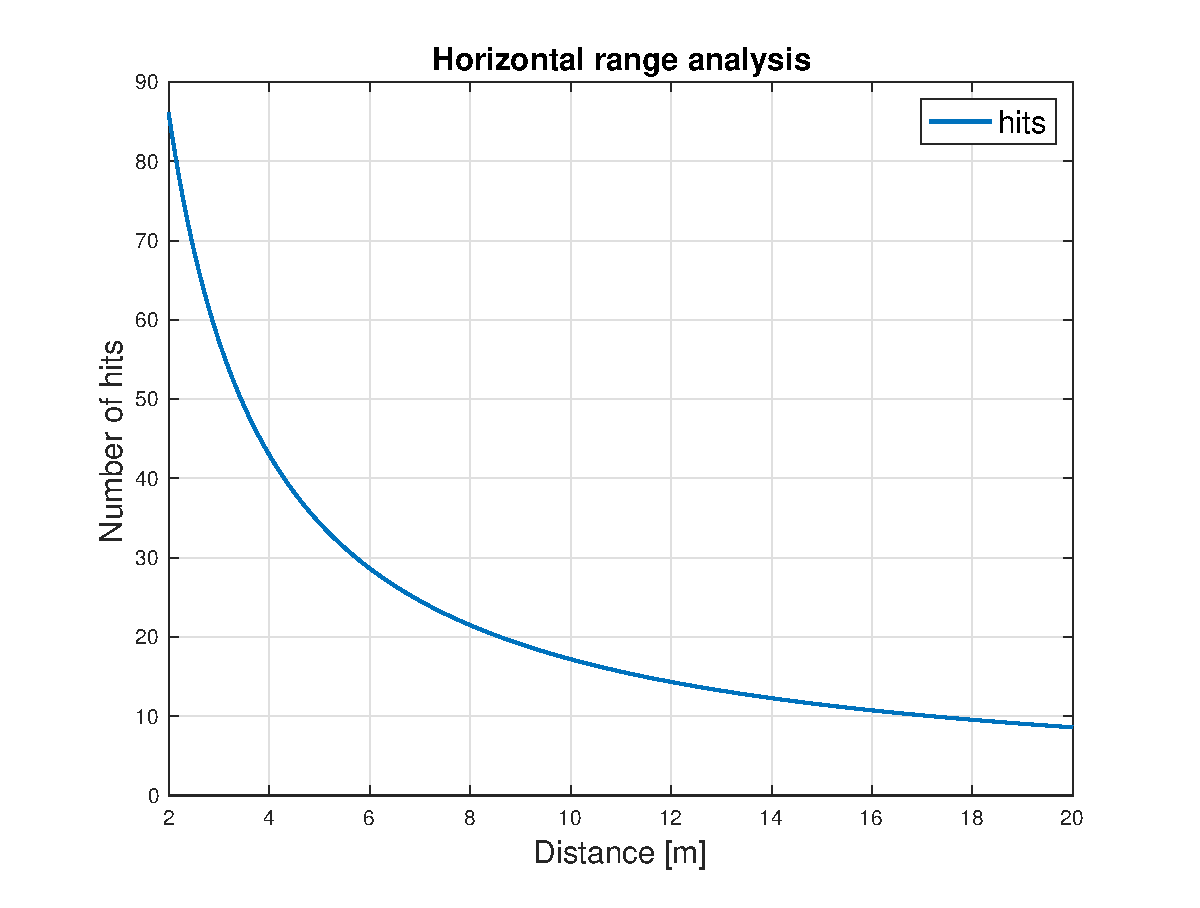
\includegraphics[scale=0.55]{fig/horizontal_range.eps}
\caption[Horizontal range chart]{Number of hits of the smallest brick from given distance.}
\label{fig:horizontal_hits}
\end{figure}

In the figure \ref{fig:horizontal_hits} is clearly visible that the horizontal resolution of the lidar is not limiting factor of the range. Even from 10 meters is lidar able to hit red brick more than 15 times. On the other hand the figure \ref{fig:vertical_hits} shows that pile of bricks with height 40 cm would be hit by less than two lidar layers from distance bigger than 6 meters. Furthermore this is the best case scenario analysis where $\beta$ is right angle which happens rarely in reality.
 
\begin{figure}[H]
\centering
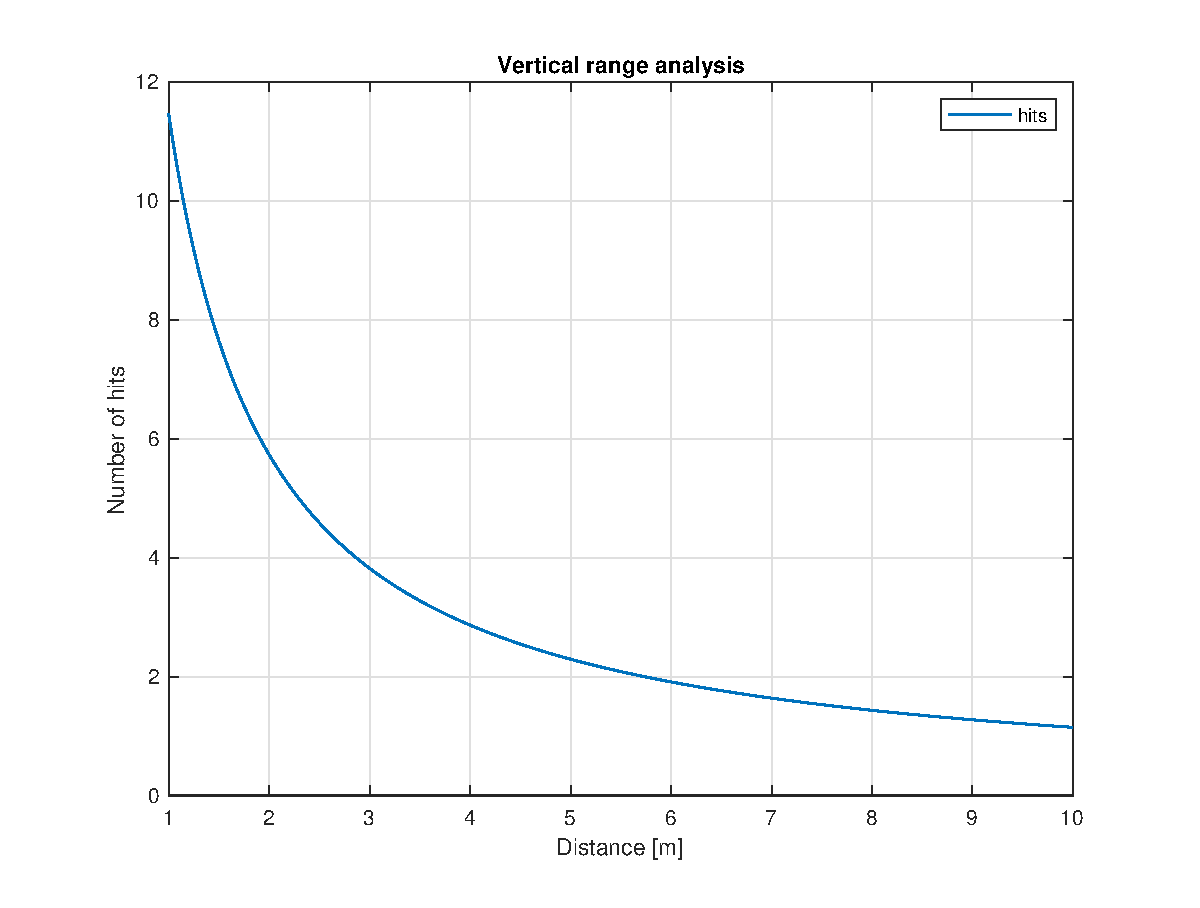
\includegraphics[scale=0.55]{fig/vertical_range.eps}
\caption[Vertical range chart]{Number of hits of two stacked bricks from given distance.}
\label{fig:vertical_hits}
\end{figure}


\section{Detection pipeline}
Detection is divided into three parts. All three parts are discussed in next three subsections. detection pipeline is visualized in the figure \ref{fig:flowchart}. 

\hspace{5px}
\begin{figure}[H]
\centering
\includegraphics[scale=0.06]{fig/flowchart.pdf}
\caption[Program pipeline]{Visualization of subsequent steps of detection.}
\label{fig:flowchart}
\end{figure}

It can be seen that the symbolic map has two types of inputs. The main advantage of this approach is that it extends the lidar detection range. As we discussed in previous section, used lidar has low vertical resolution - only 16 layers. Thus the bricks are often visible in only one layer of lidar scan. If we use only one scan, there is a high probability of false positive measurements. On the one hand we can decrease the occurrence of false positives by adding other lidar layers into the detection process. But on the other hand two layers are available only from distance smaller than 6 meters and that decreases the detection range. Therefore we exploited both approaches. One layer line segmentation for generating the candidates with low confidence and multilayer pile detector providing high quality estimates.

\section{Line segmentation}
For line segmentation is used IEPF algorithm very similar to the one described in algorithm \ref{alg:segmentation}. Only the final merging parallel segments is omitted, because it can connect two bricks into one. After retrieving the segments, a filtering based on the segment size is done. It is possible to assign the color to the segment because each brick type has unique dimensions. Example of lidar measurement with extracted and filtered lines is in the figure \ref{fig:segments}. Algorithm performance is influenced by correct setup of constants $C$ and $S$ (clustering and splitting distance). If we choose to high C, it could happen that the algorithm joins two bricks into one segment. As described in figure \ref{fig:piledef} the distance between two bricks of same color is 10 cm. Therefore the clustering distance must be always less than 10 cm. If the clustering distance is too low, one brick can be unintentionally divided into many segments and without merging at the end are these segments useless. It is necessary to bear in mind that the lidar precision as shown in table \ref{tab:lidar} is $\pm3$ cm so any clustering with distance smaller than 6 cm will be highly affected be sensor noise. The found segments are transformed into the map frame and passed to symbolic map as low confidence detections. Further are segments passed to pile detector which can filter out false positive detections.

\hspace{8mm}

\begin{figure}[H]
\centering
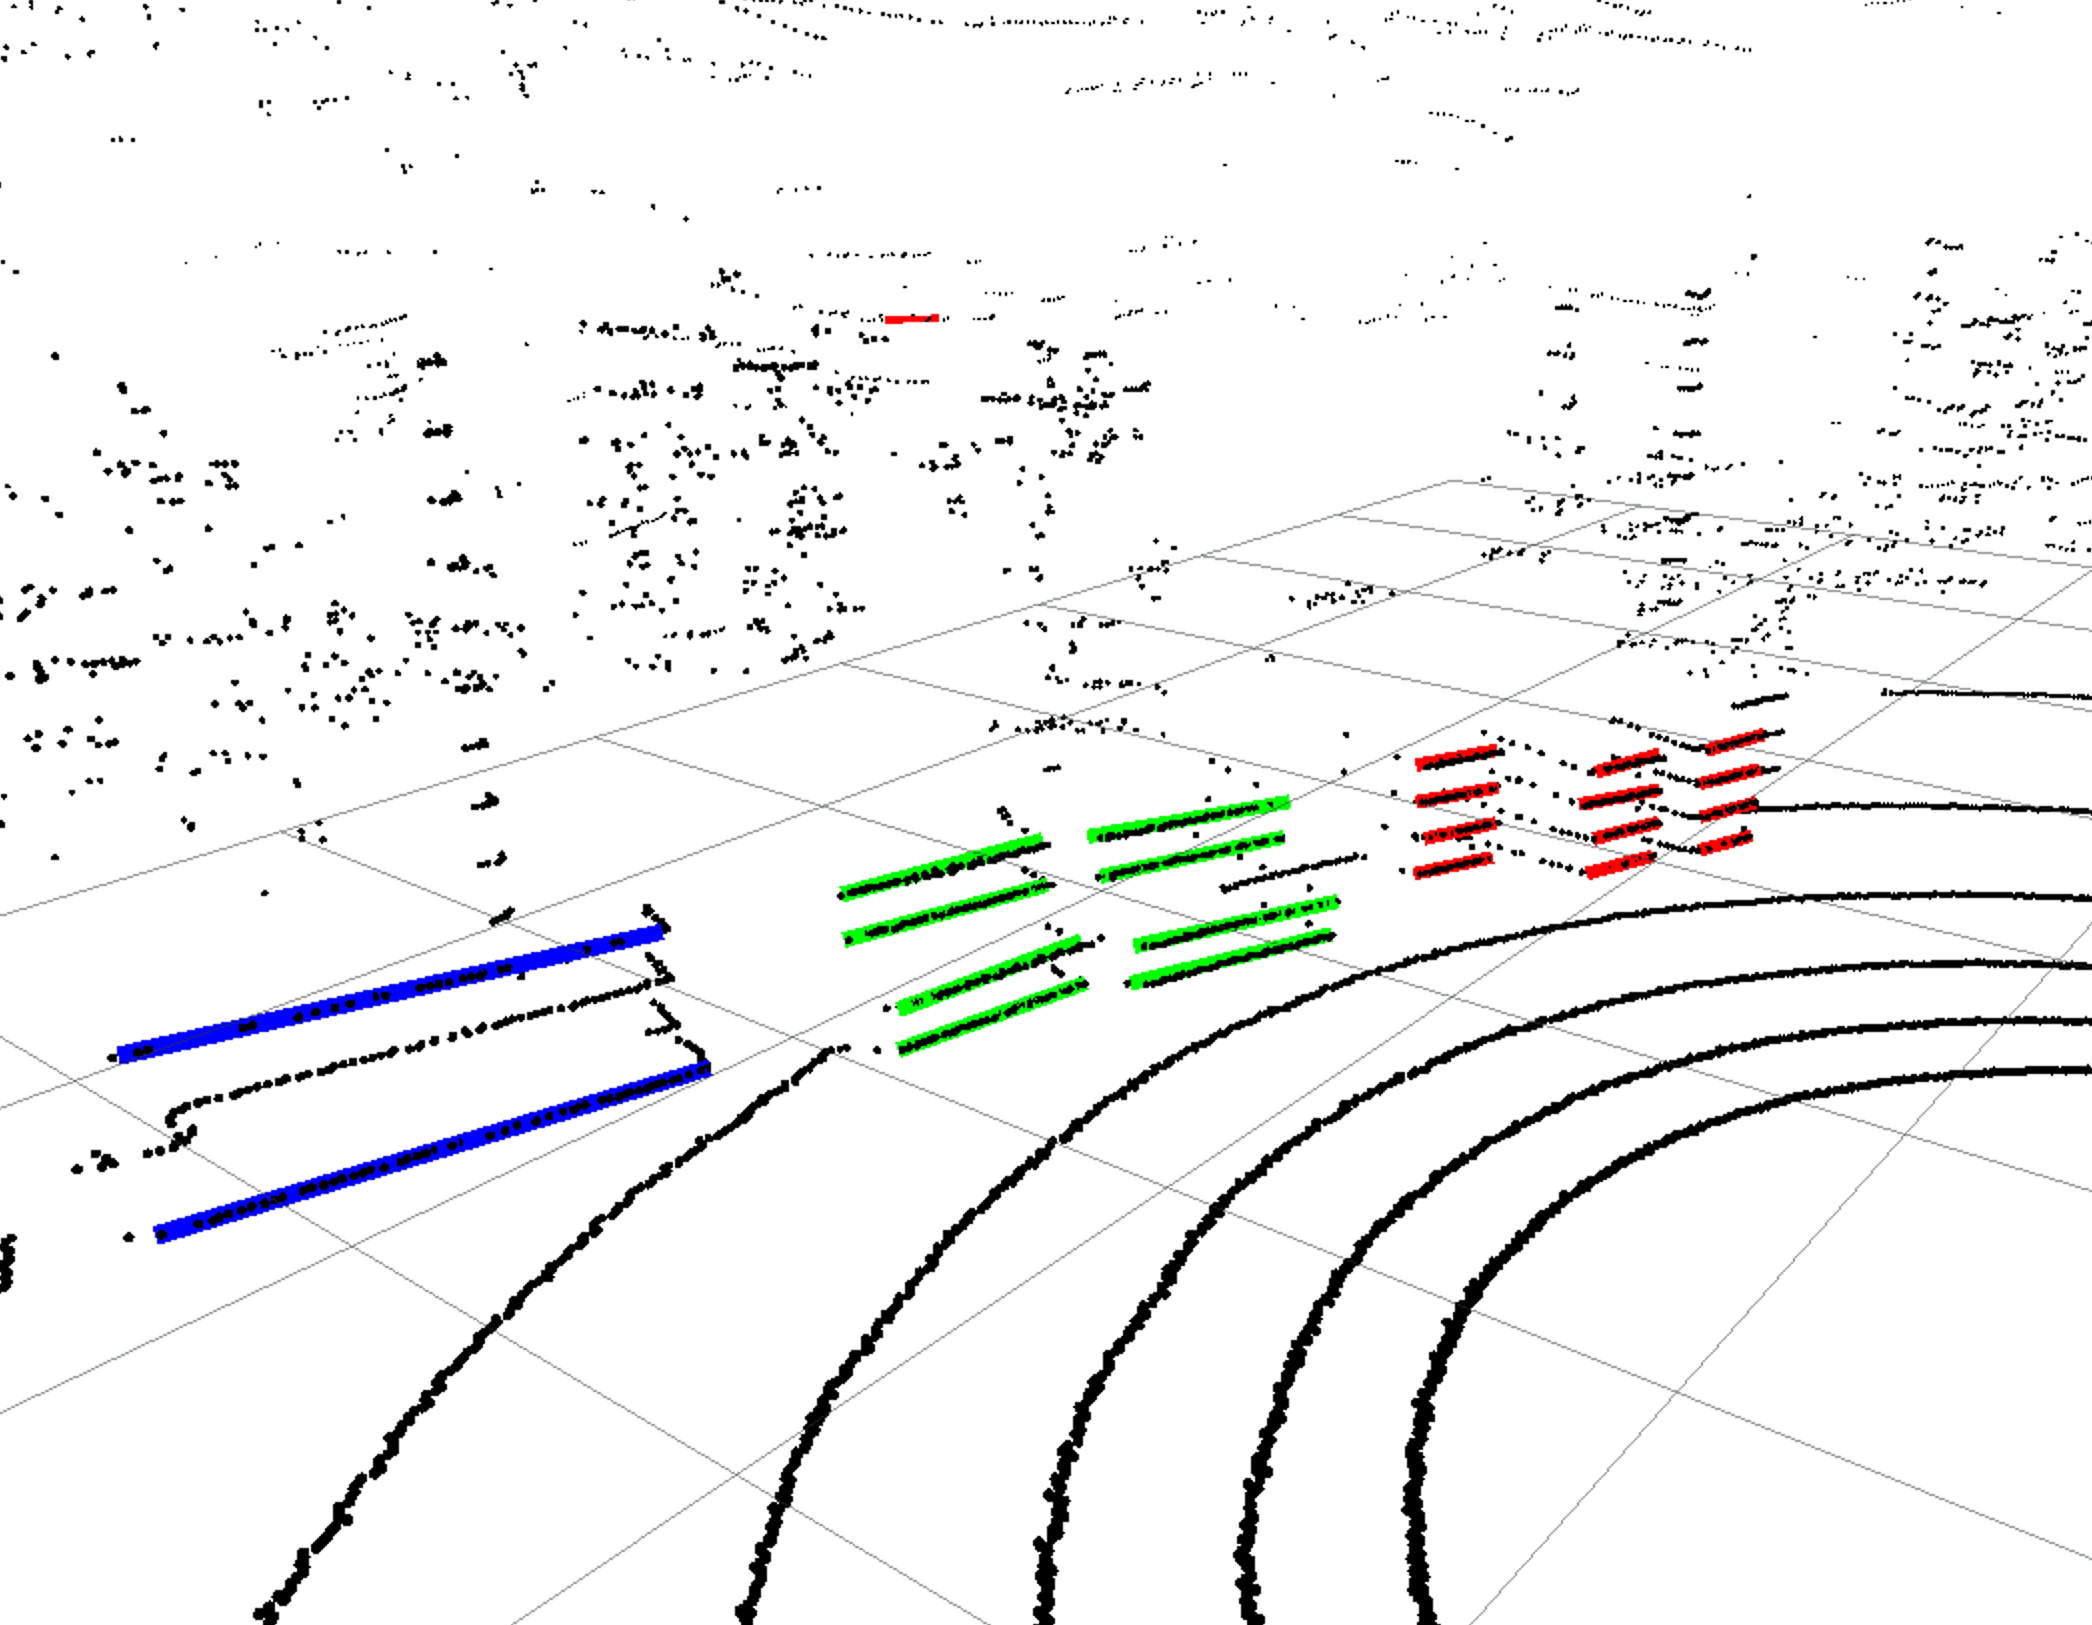
\includegraphics[scale=0.43]{fig/segments}
\caption[Line segmentation visualization]{RViz visualization of line segmentation. In the figure is evident that the bricks are well detected. This detection is done from $\approx3$m. There is visible one false positive detection behind the brick piles on a tree.}
\label{fig:segments}
\end{figure}


\section{Pile detection}
The pile detector uses one of the simplest version of EM algorithm. As a model for the pile is applied 2D multivariete Gaussian distribution with variance fixed to one. Although, this model is not precise description of the detection probability, it has other advantages already discussed in previous chapters. It is easy to work with and it converges to the global optimum very well. Only the mean value is optimized and it should converge into the center of the pile. The stopping criterion for the algorithm is solely number of iterations. The robot is realtime system and there are strict demands for meeting a deadline. There are further requirements for a hypothesis to be declared as pile after the optimization is done. We look around the proposed center in one meter radius and we inspect all bricks found in this area. All the following conditions must be fulfilled for segments in the pile:
\begin{itemize}
\item There are at least two unique heights ($z$ positions).
\item There are at least two unique places ($(x,y)$ positions).
\item Difference between maximal and minimal height is less than the pile height.
\item Pile center is inside the arena.
\end{itemize}
When these conditions are met then the hypothesis is declared as pile and pushed into symbolic map with high confidence. When one of these conditions is violated then all the segments in this hypothesis are deleted and the algorithm runs again until there are no more segments within the hypothesis radius. Whole procedure is shown in algorithm \ref{alg:pile_detection}.

\begin{algorithm}[]
 \KwData{segments}
 \KwResult{pile\_position}
\While{True}{
	pile\_position = fit\_em(segments)\;
	pile\_segments = segments\_in\_pile(pile, segments)\;
	\If{pile\_segments.size() $< 2$}{
		return None\;	
	}
	\eIf{is\_pile(pile\_segments)}{
		return pile\_position\;
	}{
		segments.delete(pile\_segments)\;
	}
} 
 \caption{Algorithm to obtain pile centers.}
 \label{alg:pile_detection}
\end{algorithm}

\begin{figure}[H]
\centering
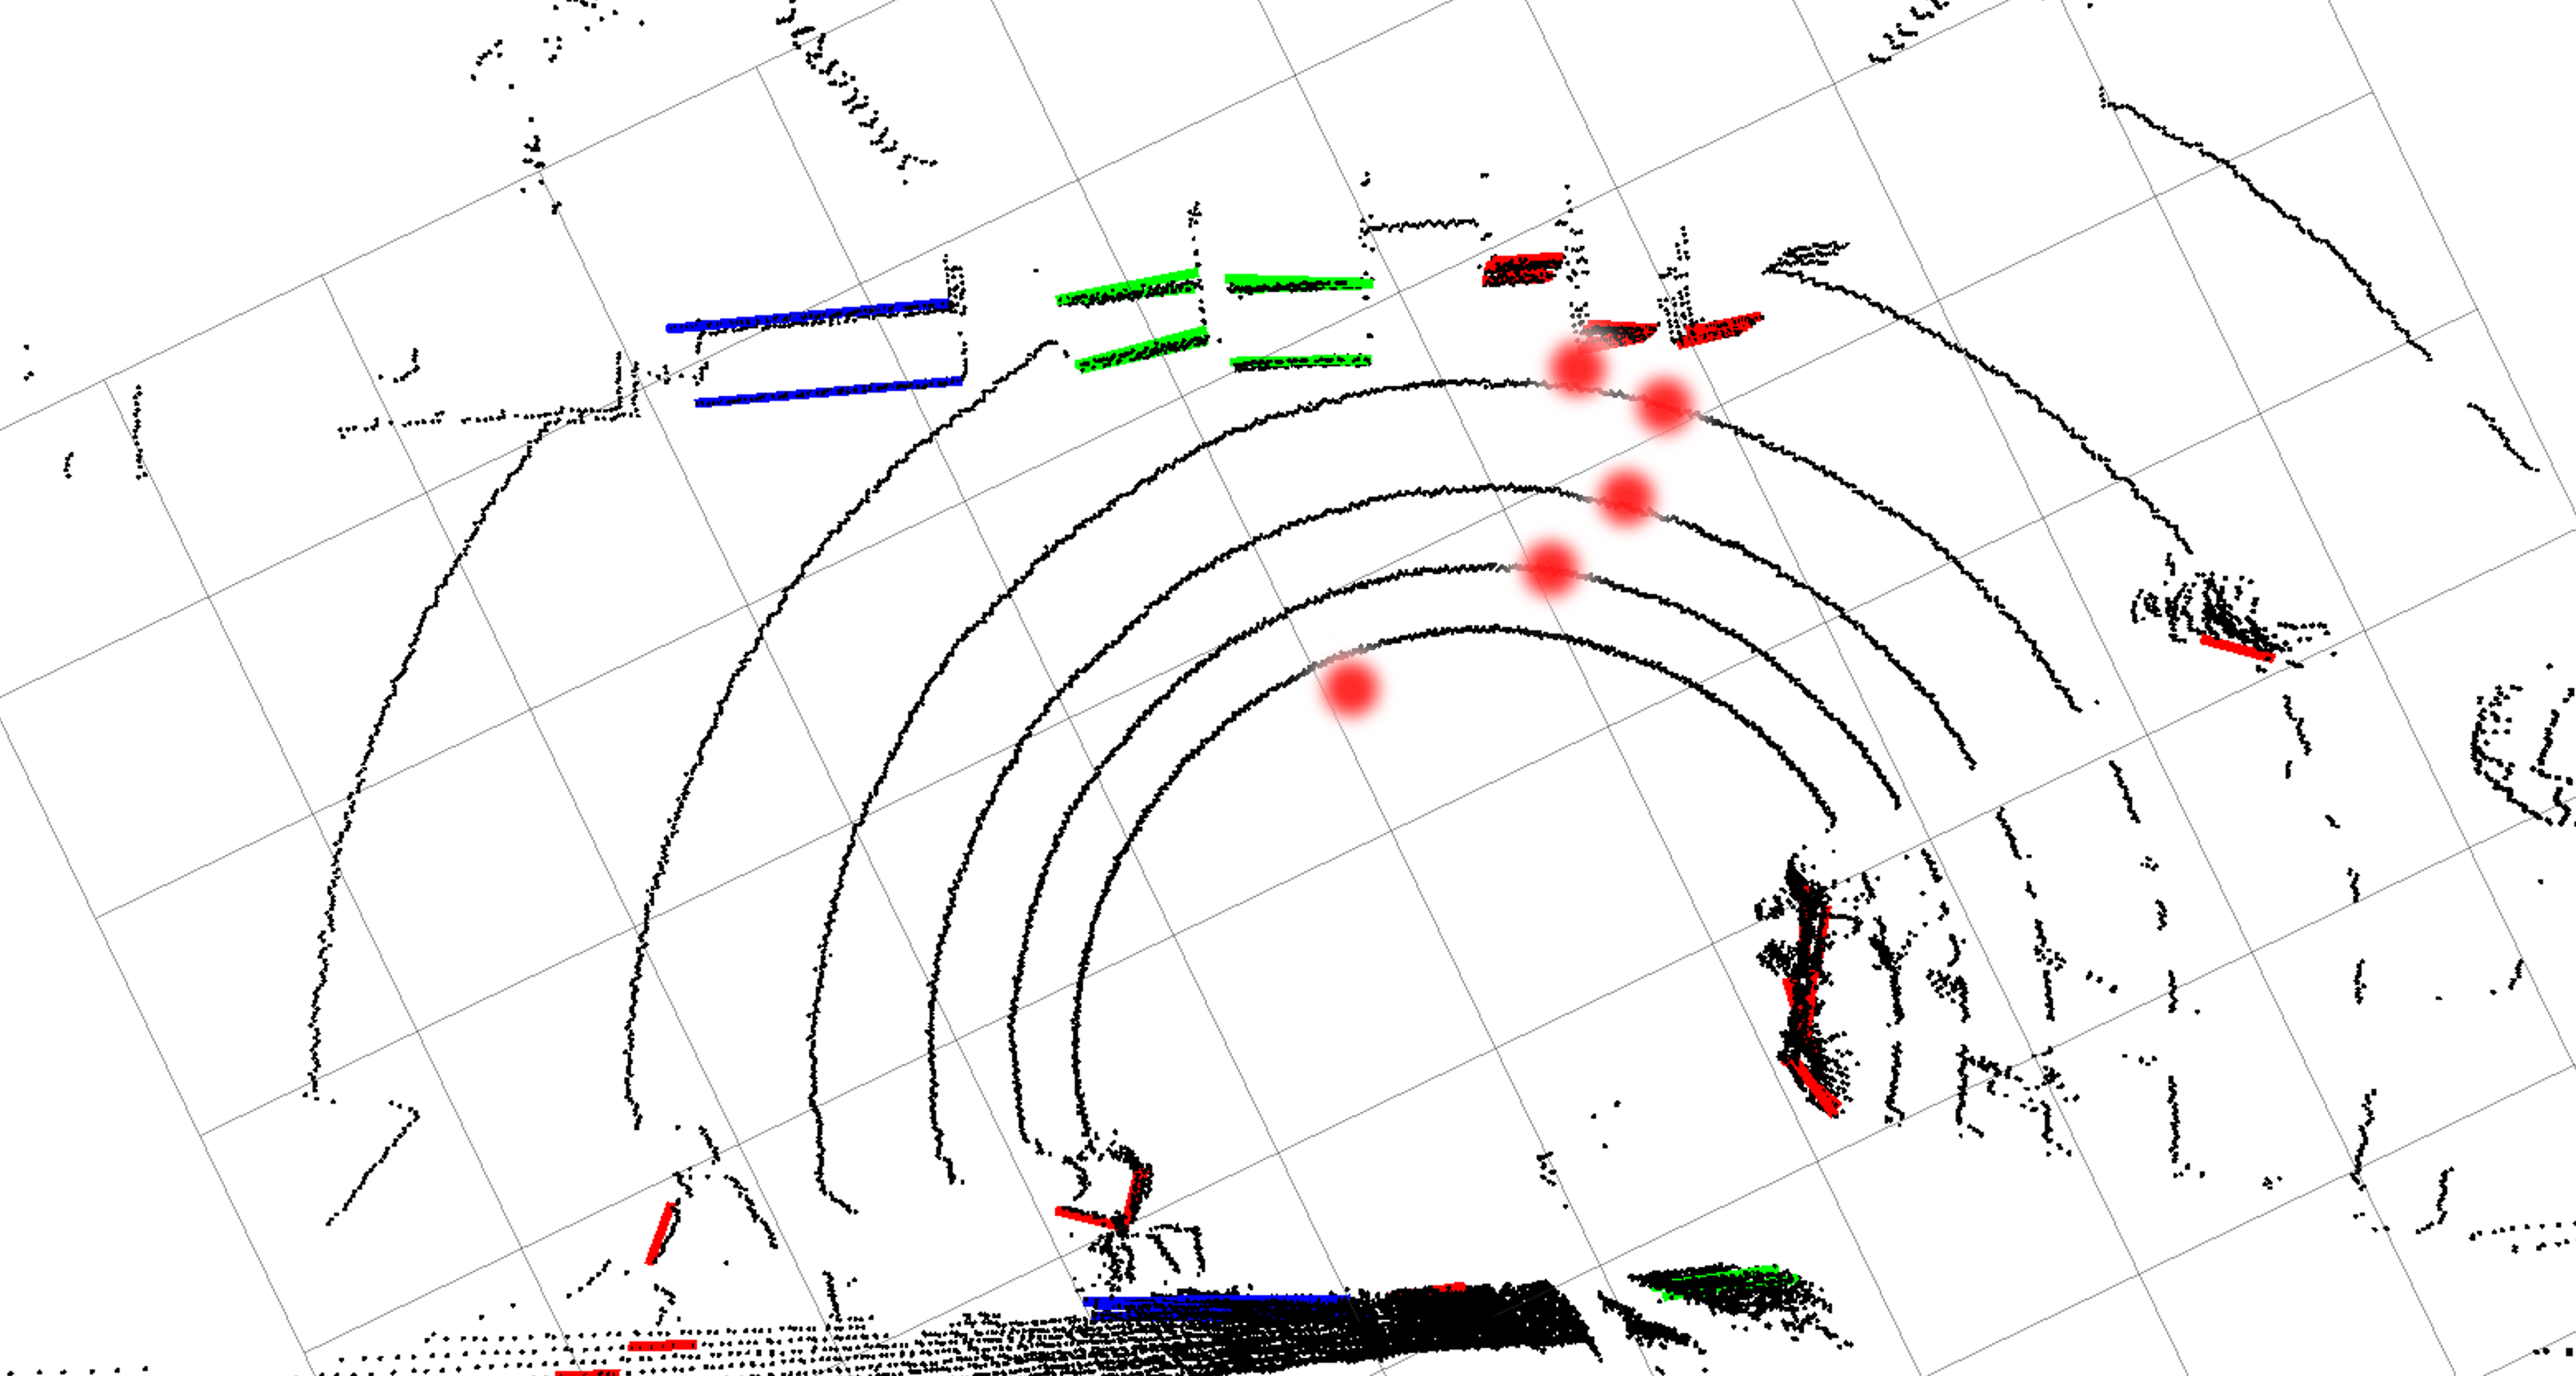
\includegraphics[scale=0.3]{fig/em_algo.png}
\caption[Em Algorithm in pile detector]{Several steps of EM algorithm for the red pile. Colored lines are the visualized segments same as in the figure \ref{fig:segments}. Red dots show subsequent positions of mean value of multivariete Gaussian. Although, there are many false positives especially in the bottom of the picture, the pile model ensures that the algorithm converges to correct place.}
\label{fig:em}
\end{figure}


\section{Pattern fitting}
Ah shown in the figure \ref{fig:flowchart} the last step of detection pipeline is pattern fitting. It is also visible that there are two types of input into this last step. Each input is used for different type of pattern fitting. In previous two sections it was described how to generate candidates with different levels of confidence. This section describes how the candidates can be used for generating actual positions and how information about the spatial distribution of bricks can be exploited for the detection. From figure \ref{fig:piledef} is known exact position of each pile and even each brick. Pattern in which are bricks stacked has three degrees of freedom - position $(x, y)$ and rotation $\phi$. Goal of the pattern fitting is to find values of these parameters in the map frame.

\subsection{Brick fitting}
The first type of fitting is using detected 3D positions of individual bricks obtained in pile detector. In the pattern is described position of each brick which can be detected by lidar sensor. Next step is to generate hypothesis which align this pattern with the measured positions of bricks. For this step is utilized the RANSAC algorithm. Firstly we draw two different bricks from detected set of bricks. Secondly the correspondences are used to find the transformation - two correspondences are enough to generate the hypothesis (rotation matrix $R$ and translation vector $t$). The brick types (colors) and brick $z$ positions are used as the correspondences. Also we know that the distance between corresponding pairs should match, otherwise it would be incorrect correspondence. Lastly we measure the cost of the hypothesis. When the bricks are stacked into the pattern with a reasonable precision, it is possible to fit the pile with average brick error down to $\pm 3$cm. After such a observation we set the inlier distance to $5$cm. Algorithm is stopped after certain number of iterations. The result is passed only if all detected bricks are inliers.

\subsubsection{Hypothesis ambiguity}
It is obvious that we cannot properly test the hypothesis when there are not enough bricks found. In addition we can see the pile from behind which renders a two different patterns to match. For this reason is required at least five detected red bricks to even start the brick fitting. As shown in the figure \ref{fig:ambiguity} even with four detected red bricks can be hypothesis easily fitted incorrectly. All conditions which can start fitting the hypothesis from front view are listed bellow:
\begin{itemize}
\item 5 red bricks detected.
\item 3 green bricks detected.
\item 4 bricks of at least two colors detected.
\end{itemize}
For view from behind is sufficient only the last condition.
\begin{figure}[H]
\centering
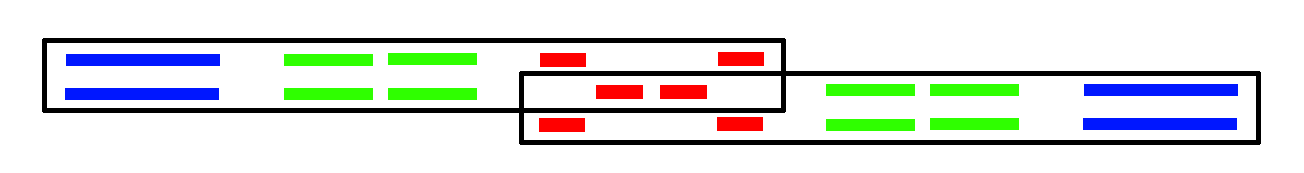
\includegraphics[scale=0.3]{fig/ambiguous.png}
\caption[Hypothesis ambiguity]{in black rectangles are visualized two possible hypothesis which can be generated by four red bricks in the intersection of rectangles. This is top view of detection from the front, so it is not visible that all red bricks are in two layers.}
\label{fig:ambiguity}
\end{figure}

\subsection{Cluster fitting}
The second type of fitting polls clusters from symbolic map and utilizes their confidence and spatial distribution. For RANSAC algorithm would be hypothesis using only four clusters too sparse to fit reliably. Because of this reason is the cluster fitting done by the EM algorithm. As in pile detection is used multivariete Gaussian distribution to represent the pile but this time the model takes in account relationships between positions of the piles. We define the probability model as follows:
\begin{equation}
P(\vec{x}_m) = \mathcal{N}_m(\vec{x}_m; \vec{\mu} + k_m\vec{v}; \bm{\Sigma}),
\end{equation}
where $m$ is pile (color) index and $M$ is absolute number of colors, $\vec{x}_m$ is measurement of color $m$, $\vec{\mu}$ is mean value of whole model, $\bm{\Sigma_m}$ is covariance matrix, $k_m$ is scalar multiplier unique for each pile and $\vec{v}$ is defined as:
\begin{equation}
\vec{v} = \begin{bmatrix}
\cos \phi \\
\sin \phi
\end{bmatrix},
\end{equation}
where $\phi$ is rotation of model. This definition of model ensures that all piles (Gaussians) are in the line with distance defined by multiplier $k$. Now we want to obtain the position and rotation of such a model based on real measurements. There is a closed form solution for maximizing both terms which can be found using maximum likelihood estimate. For mean value is derivation very similar to simple Gaussian:
\begin{align}
\frac{\partial \log\mathcal{L} }{\partial \vec{\mu}} &= \sum_{m=1}^M \bm{\Sigma}^{-1}_m \sum_{n = 1}^{N_m} (\vec{x}_{m_n} - \vec{\mu} - k_m \vec{v}) \\
\vec{\mu} &= \sum_{m=1}^M \sum_{n = 1}^{N_m} \frac{\vec{x}_{m_n} - k_m \vec{v}}{N_m}.
\end{align}
Further is necessary to derive MLE for rotation $\phi$ which is hidden inside vector $\vec{v}$. For simplicity is now the matrix equation split into one part for each of two dimensions.  
\begin{align}
\frac{\partial \log\mathcal{L}_x }{\partial \phi} &= \sum_{m=1}^{M} \frac{1}{\sigma^2_x} \sum_{n=1}^{N_m} (x_{m_n, x} - \mu_x - k_{m, x} \cos \phi) \left( -k_{m,x} \sin \phi\right)  \\
\frac{\partial \log\mathcal{L}_y }{\partial \phi} &= \sum_{m=1}^{M} \frac{1}{\sigma^2_y} \sum_{n=1}^{N_m} (x_{m_n, y} - \mu_y - k_{m, y} \sin \phi) k_{m,y} \cos \phi
\end{align}
Likelihood derivative is now set equal to zero to find the extremes for each dimension.
\begin{align}
\cos \phi &= \sum_{m=1}^{M} \frac{1}{k_{m, x}N_m} \sum_{n = 1}^{N_m} x_{m_n, x} - \mu_x \\ 
\sin \phi &= \sum_{m=1}^{M} \frac{1}{k_{m, y}N_m} \sum_{n = 1}^{N_m} x_{m_n, y} - \mu_y .
\end{align}
Now it is possible divide one equation by the other, use basic relationship of trigonometric functions and derive final expression for maximizing the rotation $\phi$:
\begin{align}
\phi &= \arctan \left( \frac{\sum_{m=1}^{M} \dfrac{\sum_{n = 1}^{N_m} \left( x_{m_n, y} - \mu_y \right)}{k_{m, y}N_m} }{\sum_{m=1}^{M} \dfrac{\sum_{n = 1}^{N_m} \left( x_{m_n, x} - \mu_x \right)}{k_{m, x}N_m} }\right).
\label{eq:prob}
\end{align}
Although the expression can be further simplified, in this form it is easier to weight each data sample by the expectation $\alpha$. Final form used in maximization step looks as follows:
\begin{align}
\phi = \arctan & \left( \dfrac{\sum_{m=1}^{M} \dfrac{\sum_{n = 1}^{N_m} \alpha_{m_n, y}(x_{m_n, y} - \mu_y)}{k_{m, y}\sum_{n = 1}^{N_m} \alpha_{m_n, y}} }{\sum_{m=1}^{M} \dfrac{\sum_{n = 1}^{N_m} \alpha_{m_n, x} (x_{m_n, x} - \mu_x) }{k_{m, x}\sum_{n = 1}^{N_m} \alpha_{m_n, x}} }\right)\\
\vec{\mu} =& \sum_{m=1}^M \dfrac{\sum_{n = 1}^{N_m}  \vec{\alpha}_{m_n} \left( \vec{x}_{m_n} - k_m \vec{v} \right) }{\sum_{n = 1}^{N_m} \vec{\alpha}_{m_n}}.
\end{align}
Method is demonstrated in the figure \ref{fig:em_pattern}. Expectation is calculated simply by evaluating the probability of sample $P(\vec{x}_m)$ as in equation \ref{eq:prob}.

\begin{figure}[H]
	\centering
	\begin{subfigure}{0.49\textwidth}
		\centering
		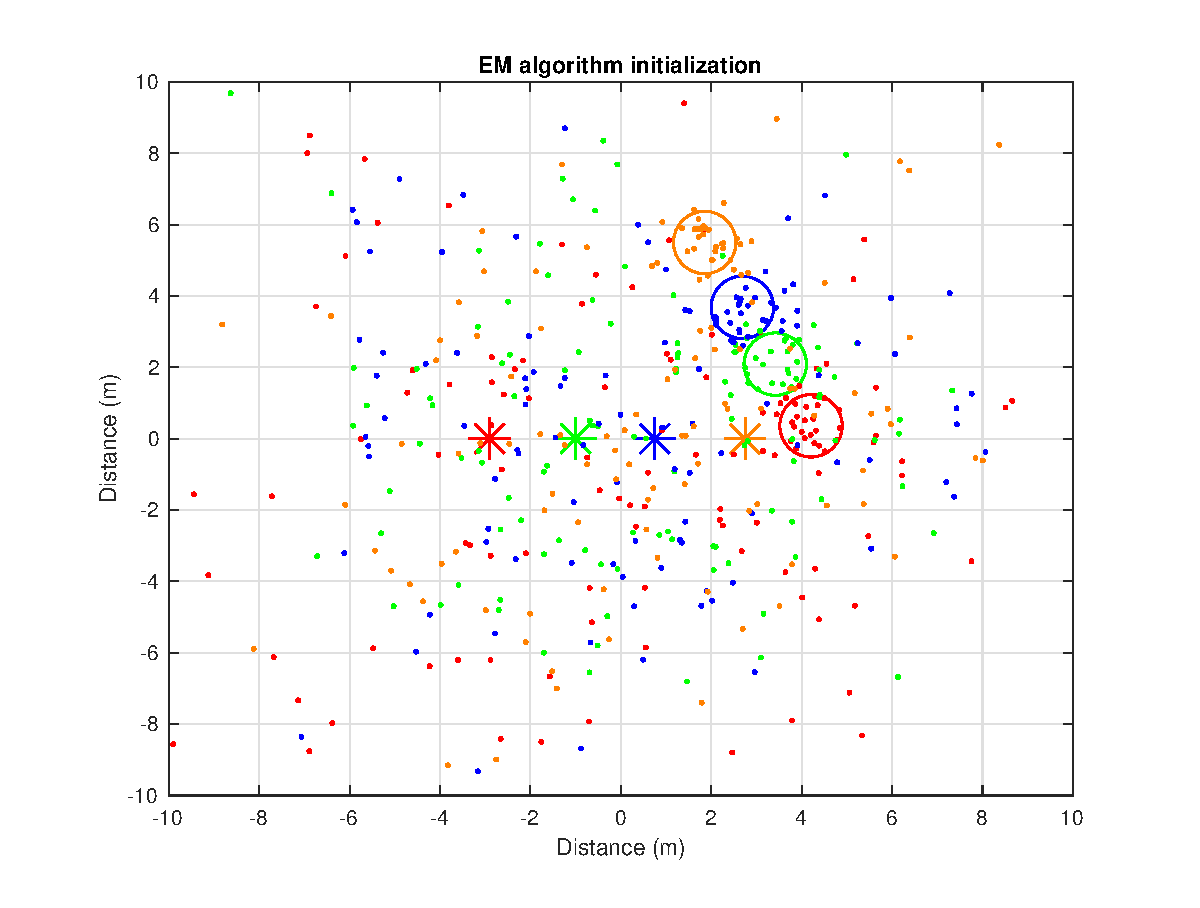
\includegraphics[scale=0.43]{fig/em_init.eps}
	\end{subfigure}
	\begin{subfigure}{.49\textwidth}
		\centering
		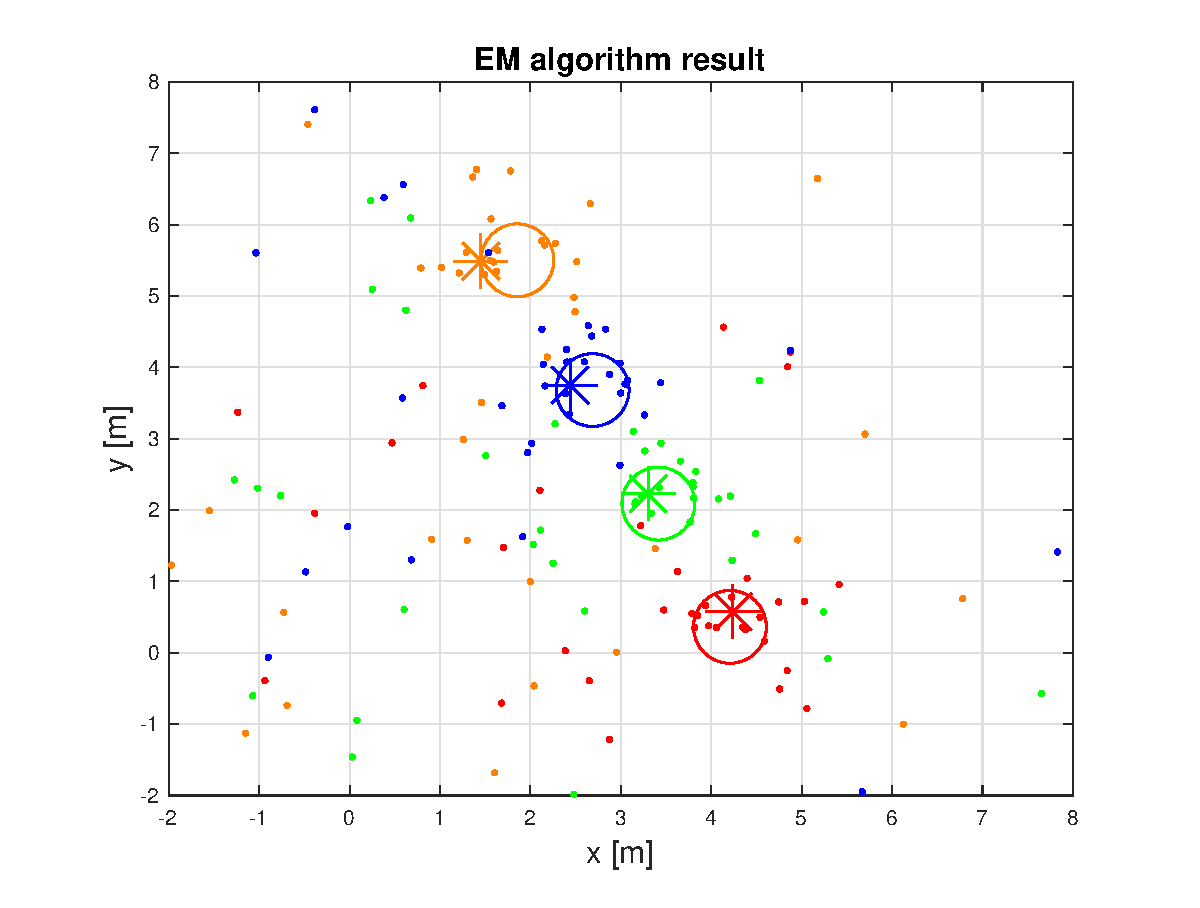
\includegraphics[scale=0.43]{fig/em_result.eps}

	\end{subfigure}
	
	\caption[EM pattern fitting]{In the pictures is visualised pattern fitting using EM algorithm. On the left is algorithm initialized with parameters $\vec{x}=(0, 0)$ and $\phi=0$. Algorithm estimate is marked by stars. Points are generated by sampling multivariete Gaussian distribution. Model was sampled with parameters $\vec{x}=(3, 3)$ and $\phi=2$ to create desired pattern of points. Positions of sampled piles are marked as circles. At the end of process are parameters found correctly.}
	\label{fig:em_pattern}
\end{figure}

\subsubsection{Convergence}
The unimodality of model's likelihood was disrupted by adding the rotation parameter to Gaussians. Possible local optimum is shown in the figure \ref{fig:em_local}. Now there are no guarantees that the algorithm will converge into the global optimum. This is common problem of EM algorithm when dealing with more complex problems. Many solutions of this issue was proposed. Very advantageous is that local optima are usually significantly worse in terms of likelihood than the global optimum. One of methods how to avoid local optima is the deterministic annealing which influences the expectation in maximization step \cite{ueda1998}. Another way how to escape local optimum is to apply the perturbations to parameters of model. In our case it could be simply rotating the model by $180\degree$. Different approach would be population based em algorithm with multiple initializations or informed initialization. The latter is easily applicable in our case because the confidences of clusters could be used as the expectation in first step.

\begin{figure}[H]
	\centering
	\begin{subfigure}{0.49\textwidth}
		\centering
		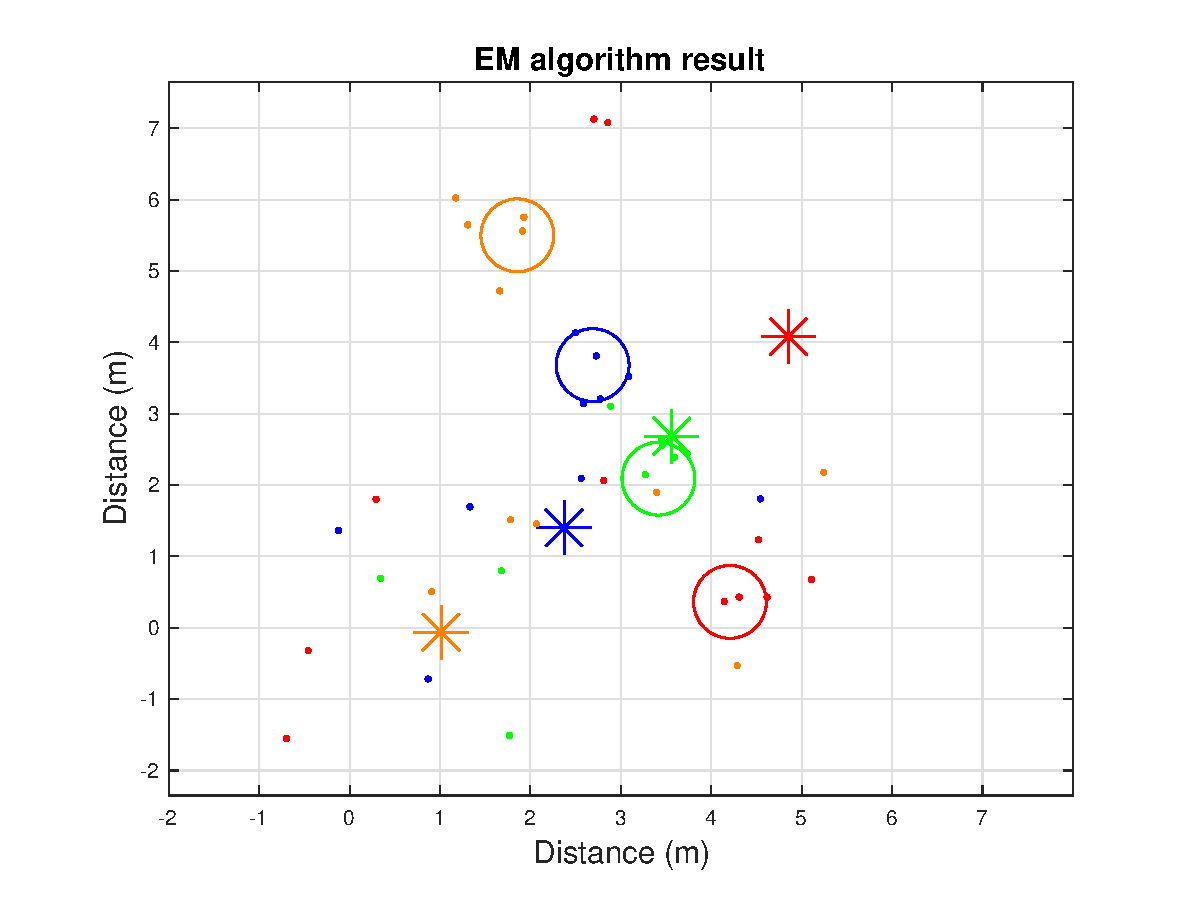
\includegraphics[scale=0.43]{fig/em_local.eps}
	\end{subfigure}
	\begin{subfigure}{.49\textwidth}
		\centering
		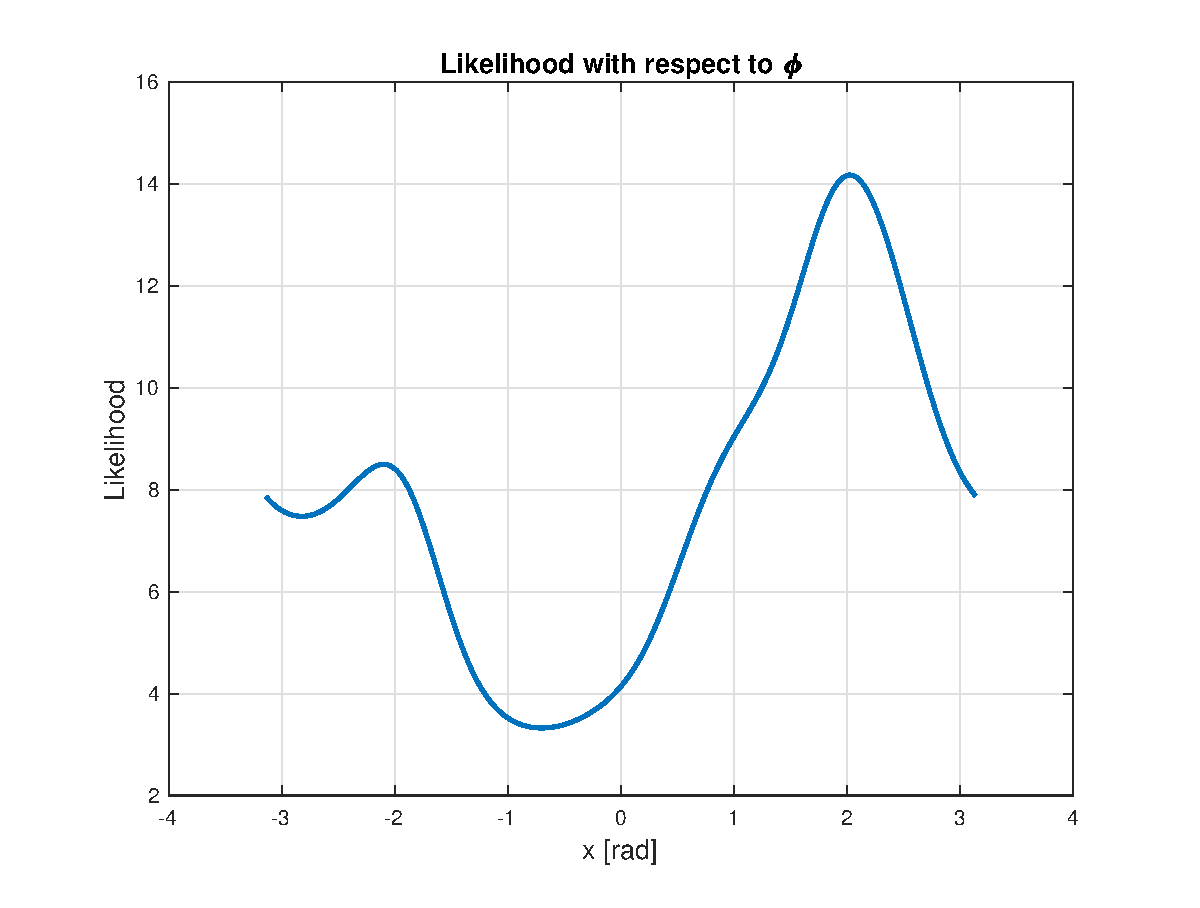
\includegraphics[scale=0.43]{fig/em_local_chart.eps}
		
	\end{subfigure}
	
	\caption[EM local optima]{When there is not enough samples the EM algorithm is more susceptible to ending in local optima as shown on the left. Right picture shows how different rotations of model with fixed mean influences the likelihood.}
	\label{fig:em_local}
\end{figure}